%% Overleaf			
%% Software Manual and Technical Document Template	
%% 									
%% This provides an example of a software manual created in Overleaf.

\documentclass{ol-softwaremanual}

% Packages used in this example
\usepackage{graphicx}  % for including images
\usepackage{microtype} % for typographical enhancements
\usepackage{amsmath}   % for equations and mathematics
\usepackage{hyperref}  % for hyperlinks
\usepackage[portuguese]{babel}
\usepackage{float}
\usepackage[a4paper,top=4.2cm,bottom=4.2cm,left=3.5cm,right=3.5cm]{geometry} % for setting page size and margins
% Custom macros used in this example document

\graphicspath{{img/}}

% Frontmatter data; appears on title page
\title{Relatório técnico do trabalho }
\version{1.0}
\author{Gustavo Lopes Rodrigues, Lucas Santiago de Oliveira}
\softwarelogo{
\includegraphics[width=8cm]{logo.png}}

\begin{document}

\maketitle

\tableofcontents
\newpage

\section{Introdução}

Esse programa feito para a disciplina de Computação gráfica, tem como objetivo integrar
C++, Qt e OpenGL, para fazer uma aplicação que seja capaz de abrir arquivos .off (Object File Format),
e ter a capacidade de manipulá-los. O programa em grande parte consiste na implementação do artigo 
\emph{"Interactive Graphics Applications with OpenGL Shading Language and Qt"}, com apenas algumas 
melhoras a sua interface, e a adição a uma funcionalidade de melhoria, que é a leitura de malhas
mistas.

\section{Organização do código}

Como dito anteriormente, utilizamos C++ como a linguagem de programação, o Qt como o framework para 
construir a interface visual na qual o usuário interage com, e o OpenGL, é a API gráfica que renderiza
os objetos, processa shaders e texturas. As seções a seguir seram separadas da seguinte forma: primeiro
apresentaremos a comunicação entre a interface visual do Qt e o código, e em seguida iremos apresentar o código 
em si e sua estruturação 

\subsection{Qt}

\begin{figure}[ht]
    \centering
    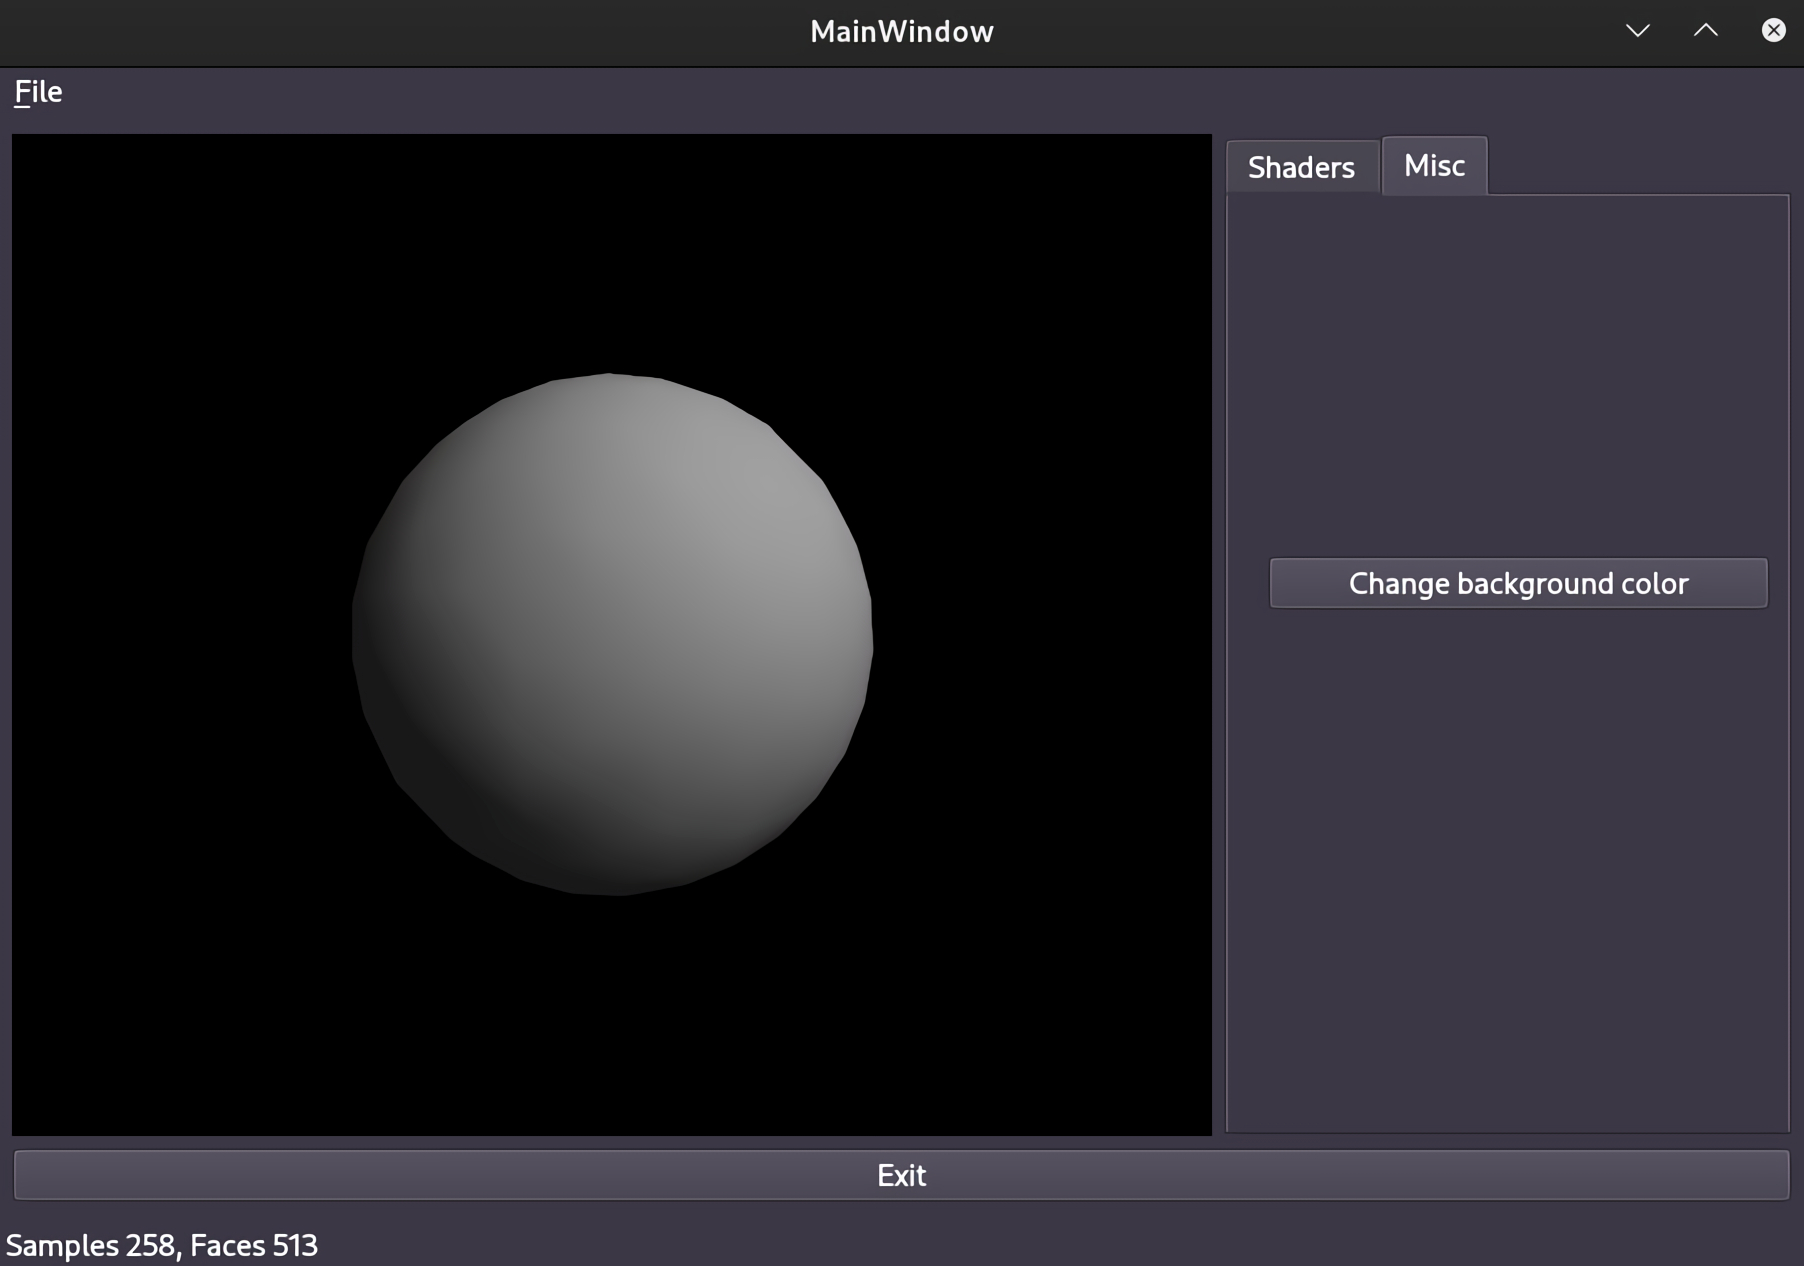
\includegraphics[width=.4\textwidth]{Interface.jpg}
    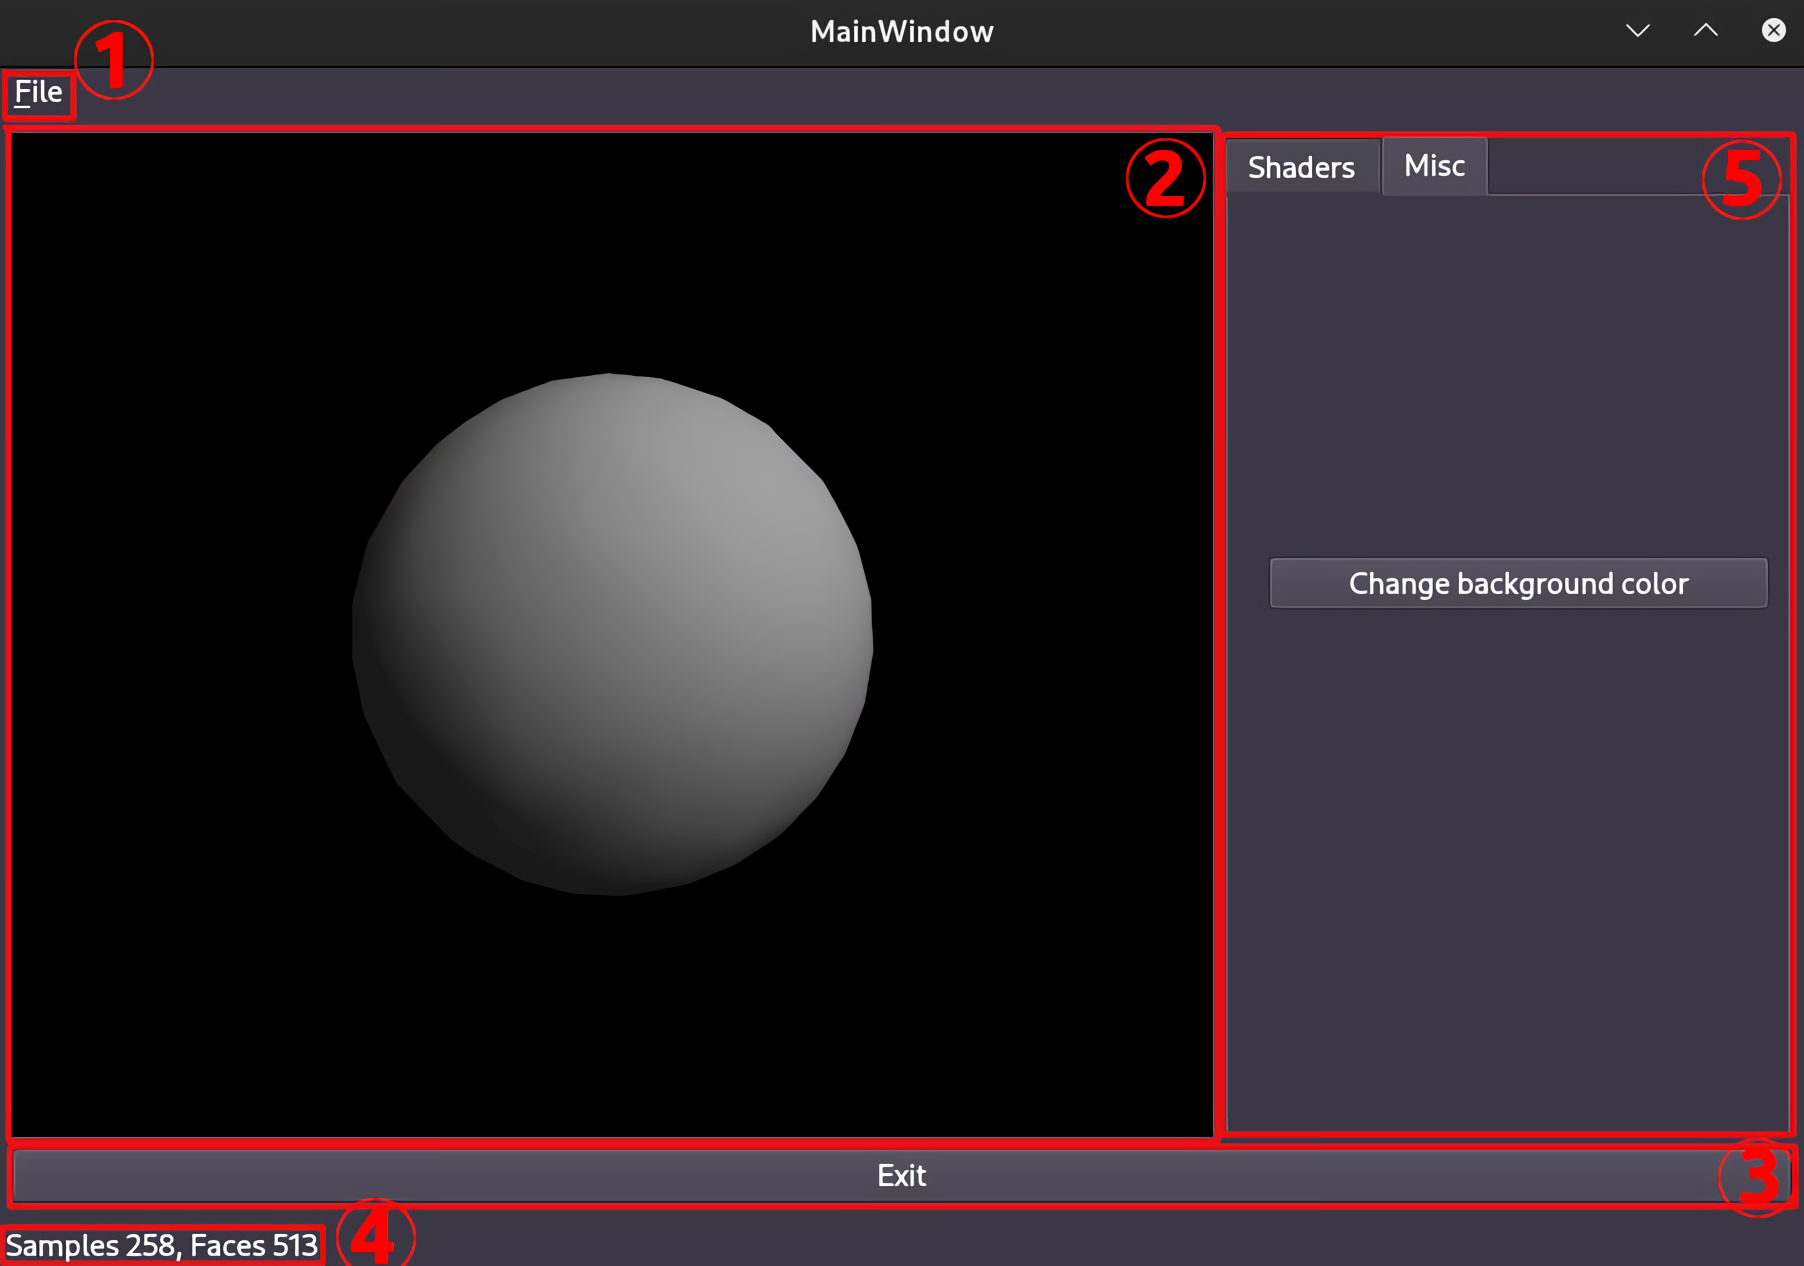
\includegraphics[width=.4\textwidth]{Interfacemarcada.jpg}
    \caption{Principal interface do programa, e a direita temos a mesma interface porém
    com marcações para sinalizar os principais componentes}
\end{figure}

A área de interação do Qt é composta de Widgets, desde os botões, até o canvas 
do OpenGL, todos os elementos são Widgets que podem ser dimensionados na tela e 
mais importante, podem usar sinais para comunicar entre-si.

\subsubsection{File}

Primeiro temos um QMenuBar, responsável em expandir e mostrar as duas
opções presentes:

\begin{itemize}
    \item \textbf{Open} - Um QMenu com um QAction, um sinal conectado
    com o visualizador dos objetos(GLWidget). Quando acionado(triggered), realiza
    a ação de abrir o gerenciador de arquivos e abrir um arquivo .off.
    \item \textbf{Screenshot} - Também um QMenu com um QAction, que conecta 
    ao GLWidget. Quando acionado(triggered), realiza a ação de abrir o gerenciador de arquivos
    e permitir o usuário salvar o frame atual do GLWidget como uma imagem .png.
\end{itemize}

\begin{figure}[H]
    \centering
    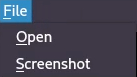
\includegraphics[width=.2\textwidth]{File.jpg}
    \caption{O botão \textbf{File} quando expandido}
\end{figure}

Além disso, o QMenuBar possui \textbf{Keybinds}, atalhos com o teclado do usuário, 
permitindo com que todas as iterações com o QMenuBar seja mais rápida, eis a seguir 
os keybinds implementados:

\begin{itemize}
    \item \textbf{Alt + f} $\rightarrow$ clicar no botão \emph{File}
    \begin{itemize}
        \item \textbf{Alt + f + o} $\rightarrow$ abrir um arquivo 
        \item \textbf{Alt + f + s} $\rightarrow$ salvar uma captura de tela 
    \end{itemize}
\end{itemize}

\newpage

\subsubsection{Visualizador de Objetos 3D}

O principal componente da aplicação, a janela onde os objetos 3D 
são exibidos é um GLWidget, onde a grande parte da implementação da 
API do OpenGL.

Esta janela é o componente que também possui a grande parte do código 
implementado, e isso inclui todo processo dos objetos, texturas e shaders, 
além de leitura de entradas do teclado e mouse do usuário. 

\begin{figure}[H]
    \centering
    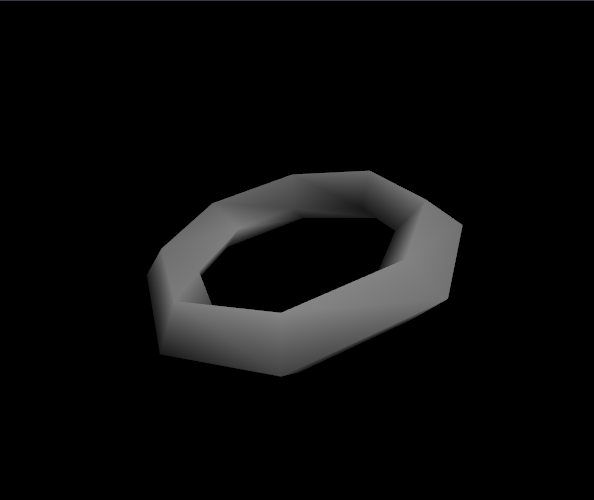
\includegraphics[width=.5\textwidth]{opengl.png}
    \caption{Objecto \textbf{octtorus.off} quando carregado}
\end{figure}

Entraremos em mais detalhe sobre os inputs do teclado e mouse, mas vamos
brevemente comentar quais são as possíveis entradas.

\textbf{Teclado:}

\begin{itemize}
    \item \textbf{Número 1 do teclado} $\rightarrow$ aplicar o algoritmo de \emph{Gouraud}
    \item \textbf{Número 2 do teclado} $\rightarrow$ aplicar o algoritmo de \emph{Phong}
    \item \textbf{Número 3 do teclado} $\rightarrow$ aplicar uma \emph{Texture}
    \item \textbf{Número 4 do teclado} $\rightarrow$ aplicar uma textura com \emph{Normal}
    \item \textbf{Esc} $\rightarrow$ fechar a aplicação
\end{itemize}

\textbf{Mouse:}

\begin{itemize}
    \item \textbf{Scroll} - Realizar ampliação(zoom) no objeto 
    atualmente selecionado. 
    \item \textbf{Botão direito + movimentar o mouse} - Realizar uma operação 
    de rotação no objeto.
\end{itemize}

\subsubsection{Botão de saída}

QPushButton widget que possui um sinal ligado a janela principal do programa,
pedindo o mesmo para o programa ser fechado.

\begin{figure}[H]
    \centering
    
\includegraphics[width=\textwidth]{botao-saida.png}
    \caption{O botão para sair do programa}
\end{figure}

\subsubsection{Barra de status}

Uma barra de status que fica no canto inferior da tela, 
informando usuários de quantos samples e faces foram carregadas 
do objeto 3D.

Este possui um sinal ligado ao GLWidget, que recebe do mesmo, 
uma QString, com as informações mencionadas.

\begin{figure}[H]
    \centering
    
\includegraphics[width=.3\textwidth]{status-bar.png}
    \caption{Barra de status com informações do \textbf{octtorus.off}}
\end{figure}

\newpage

\subsubsection{Abas de edição}

\begin{figure}[H]
    \centering
    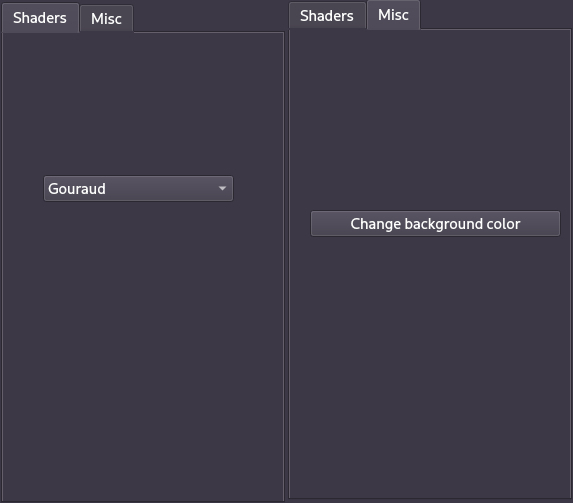
\includegraphics[width=.5\textwidth]{abadeedicao.jpg}
    \caption{As duas abas de edição}
\end{figure}

Para armazenar as possíveis, utilizamos um gerenciador 
de abas(QTabWidget), que armazenará duas abas(QWidget): uma 
responsável em guardar operações com shaders, e outra 
para trocar cor do fundo do GLWidget.

\begin{itemize}
    \item \textbf{Shaders} - Possui QComboBox, que apresenta 
    varios textos com nome dos possíveis shaders no 
    programa. Após selecionar um, será acionado um sinal 
    que será enviado para o GLWidget, pedindo para mudar 
    para o shader especificado pelo usuário.
    \item \textbf{Misc} - Possui um QPushButton, que acionará a 
    paleta de cor do Qt, permitindo que o usuário escolha 
    uma cor, para ser a nova cor do fundo.(mais informações 
    na seção do código)
\end{itemize}

\subsection{Código}

Agora que a comunicação na interface do Qt foi detalhada,
podemos passar a explicar a comunicação dentro do código em si.




\section{Detalhando módelos matemáticos}

\end{document}
